\section{Decision trees}

\begin{enumerate}
\item Concrete sample training data.
  \begin{enumerate}
  \item The sample entropy $H(Y)$ is $0.993$.
    \begin{align*}
      H(Y) =&\; -P(Y=+) log_2P(Y=+) - P(Y=-) log_2P(Y=-)\\
      =&\; -(22/40)log_2(22/40)-(18/40)log_2(18/40)\\
      =&\; (22/40)log_2(40/22)+(18/40)log_2(40/18)\\
      =&\; 0.993
    \end{align*}

  \item The information gains are $IG(X_1) = 0.016$ and $IG(X_2) = 0.025$.  
    \begin{align*}
      IG(X_1) =&\; H(Y)-H(Y|X_1)\\ =&\;0.993-9/40log_2(9/19)-10/40log_2(10/19)-13/40log_2(13/21)-8/40log_2(8/21)\\
      =&\;0.016\\
      IG(X_2) =&\; H(Y)-H(Y|X_2)\\ =&\;0.993-7/40log_2(7/16)-9/40log_2(9/16)-15/40log_2(15/24)-9/40log_2(9/24)\\
      =&\;0.025\\
    \end{align*}

  \item The decision tree that would be learned is shown in Figure
    \ref{fig:decision_tree}.
    %% The [H], in combination with the float package, forces latex to
    %% generate the figure in exactly this part of the document
    %% instead of ``floating'' it to another part.
    \begin{figure}[H]
      \centering
      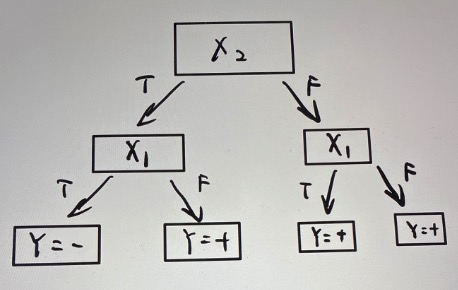
\includegraphics[width=0.4\textwidth]{images/decision_tree.png}
      \caption{The decision tree that would be learned.}
      \label{fig:decision_tree}
    \end{figure}
  \end{enumerate}

\item Information gain and KL-divergence.
\begin{enumerate}
	\item If variables $X$ and $Y$ are independent, is $IG(x,y) = 0$? If yes, prove it. If no, give a counter example.
	
	
	Yes, $IG(x,y) = 0$. Since $X$ and $Y$ are independent: 
	$$p(x, y) = p(x)p(y) \implies log\bigg(\frac{p(x)p(y)}{p(x,y)}\bigg)=log(1)=0$$
	Thus:
	$$IG(x, y)=-\sum_{x}\sum_{y}p(x, y) \times log\bigg(\frac{p(x)p(y)}{p(x,y)}\bigg)=0$$.\\
	\\
	\newpage
	\item Prove that $IG(x,y) = H[x] - H[x \mid y] = H[y] - H[y \mid x]$,
	starting from the definition in terms of KL-divergence:
	\begin{align*}
	IG(x,y) =&\; KL\left(p(x,y)||p(x)p(y)\right) \\
	=&\; -\sum_x\sum_yp(x, y)log\bigg(\frac{p(x)p(y)}{p(x,y)}\bigg)\\
	=&\; -\sum_x\sum_yp(x, y)\bigg[log(p(x))+log\bigg(\frac{p(y)}{p(x,y)}\bigg)\bigg]\\
	=&\; -\sum_x\sum_yp(x,y)log(p(x)) + \sum_x\sum_yp(x, y)log\bigg(\frac{p(x,y)}{p(y)}\bigg)\\
	=&\; -\sum_xp(x)log(p(x)) + \sum_y\sum_xp(x|y)p(y)log(p(x|y))\\
	=&\; -\sum_xp(x)log(p(x)) + \sum_yp(y)\sum_xp(x|y)log(p(x|y))\\
	=&\; H[x] - H[x \mid y]\\
	\end{align*}
	\begin{align*}
	IG(x,y) =&\; KL\left(p(x,y)||p(x)p(y)\right) \\
	=&\; -\sum_x\sum_yp(x, y)log\bigg(\frac{p(x)p(y)}{p(x,y)}\bigg)\\
	=&\; -\sum_x\sum_yp(x, y)\bigg[log(p(y))+log\bigg(\frac{p(x)}{p(x,y)}\bigg)\bigg]\\
	=&\; -\sum_x\sum_yp(x,y)log(p(y)) + \sum_x\sum_yp(x, y)log\bigg(\frac{p(x,y)}{p(x)}\bigg)\\
	=&\; -\sum_yp(y)log(p(y)) + \sum_x\sum_yp(y|x)p(x)log(p(y|x))\\
	=&\; -\sum_yp(y)log(p(y)) + \sum_xp(x)\sum_yp(y|x)log(p(y|x))\\
	=&\; H[y] - H[y \mid x]
	\end{align*}
\end{enumerate}

\end{enumerate}
